\scanpage{41}
Fujii Guruji \unsure{Nichidatsu|Nichidathu}

$I$ ens ordonné fini

$\forall i\in I\qquad V_i^\circ$ variété à bord [bord vide si $i$ minimal)

\[
\forall(i,j)\in I\times I,\quad j<i\qquad
\underset{\substack{\text{sous-}\\\text{variété à bord}}}{\partial_jV_i^\circ}\subset\partial V_i^\circ
\]
\diagram{\begin{tikzcd}
\partial_jV_i^\circ\arrow[r]&V_j^\circ
\end{tikzcd}}
\uline{fibration}

fibres des variétés à bord (variétés \inserted{sans bord} si $j$ prédécesseur de $i$)

\diagram{\begin{tikzcd}
\partial V_i^\circ=\displaystyle\bigcup_{\substack{j\in\Phi_i\\\text{ens des facettes de }i}}\underbracket{\partial_jV_i^\circ}\arrow[dr] &\\
&V_j^\circ
\end{tikzcd}}
\[
\partial(\partial_jV_i^\circ)=[(\partial_jV_i^\circ)|\partial V_j^\circ]\cup
\underbracket{\partial_{\unsure{i|\ell}/j}(\partial_jV_i^\circ)}_{\substack{\text{fibré des}\\\text{bords}}}
\]
\[
\partial(\partial_jV_i^\circ)=\bigcup_{k\in\Phi_j}\underbracket{(\partial_jV_i^\circ)|\partial_kV_j^\circ)}_{\text{fibré sur }V_k^\circ}
\cup\underbracket{\partial_{i/j}(\partial_jV_i^\circ)}_{\substack{\text{fibré sur}\\V_j^\circ}}
=\left(\bigcup_{k<j}\underbrace{(\partial_jV_i^\circ|\partial_kV_j^\circ)}_{\text{fibré sur }V_{\unsure{k|h}}^\circ}\right)
\cup\underbracket{\partial_{\unsure{0|i}/(j)}\partial V_i^\circ}_{\text{fibré sur }V_j^\circ}
\]
\figure{\begin{tikzpicture}[x=1cm,y=1cm]\node[draw,ellipse] at (0,0) {\unsure{bien|bon}};\node[anchor=west] at (.65,0) {vide si $j$ prédécesseur de $i$};\end{tikzpicture}}
\[
\partial(\partial_{j'}V_i^\circ)=\left(\bigcup_{k<j'}\partial_{j'}V_i^\circ|\partial_kV_{\unsure{j'|j}}^\circ\right)\cup
\underbracket{\partial_{i/j'}V_i^\circ}_{\substack{\text{vide si }j'\text{ préd.}\\\text{de }i}}
\]

\deleted{$\unsure{V_0|\partial_0}$}
\diagram{\begin{tikzcd}[column sep=large,row sep=small]
V_0^\circ&V_1^\circ&V_2^\circ\\
&\partial V_1^\circ\arrow[ul]&\partial V_2^\circ\arrow[d,equal]\\
&&\partial_1V_2^\circ\cup\partial_0V_2^\circ\arrow[uul,bend left=20]\arrow[uull,bend left=65]
\end{tikzcd}}
\[
\partial(\partial_0V_2^\circ)\simeq\partial(\partial_1V_2^\circ)=\partial_1V_2^\circ|\partial V_1^\circ
\]
\[
\partial_jV_i^\circ|\partial_kV_j^\circ=\partial_{j,\unsure{k|h}}V_i^\circ\qquad\text{fibré sur }V_{\unsure{h|k}}^\circ
\]
\figure{\begin{tikzpicture}[x=1cm,y=1cm]\draw[densely dashed] (0,.2)--(.65,.2);\draw[densely dashed] (.1,0)--(.8,0);\draw[densely dashed] (1.2,0)--(1.8,0);\draw (2.3,.02)--(2.4,-.02)--(2.5,0);\end{tikzpicture}}
\[
\partial_{j\unsure{>|,}h>\ell}=\partial_{j,h}V_i^\circ|\partial_\ell V_h^\circ\qquad\text{fibré sur }V_\ell^\circ
\]
\[
\partial_{j>h>\ell>m}V_i^\circ
\]

\diagram{\begin{tikzcd}[column sep=small,row sep=large]
\partial_2&\partial_{21}\arrow[l]\arrow[dr]&\partial_{20}\arrow[ll,bend right=50]\arrow[ll,bend left=20]\arrow[ddl,bend right=25]&\partial_{210}\arrow[l]\arrow[ll,bend right=50]\arrow[d,equal,"\text{bord commun}"]\\
\partial_1&\partial_{10}\arrow[l]\arrow[d,bend left=35]&\overset{\bullet\,\cdot}{\partial_{\deleted{\unsure{0}}\unsure{12|012}}}\arrow[ll,bend left=20]&\partial_{10}\arrow[l]\arrow[lll,bend left=40]\\
\partial_0&\deleted{\unsure{\partial}}\partial_0^\bullet\arrow[l]&&\text{bord commun}
\end{tikzcd}}

\figure{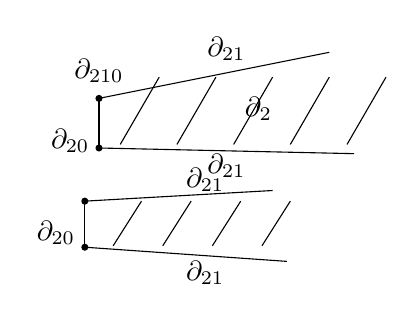
\begin{tikzpicture}[x=1cm,y=1cm,scale=.9]
\draw (0,2.8)--(3.25,3.45);\draw (0,2.1)--(3.6,2.02);\draw (0,2.8)--(0,2.1);
\foreach \x in {.3,1.1,1.9,2.7,3.5}{\draw (\x,2.15)--(\x+.55,3.1);}
\fill (0,2.8) circle(.05);\fill (0,2.1) circle(.05);
\node[above] at (0,2.88) {$\partial_{210}$};\node[left] at (0,2.2) {$\partial_{20}$};\node[above] at (1.8,3.2) {$\partial_{21}$};\node at (2.25,2.65) {$\partial_2$};\node[below] at (1.8,2.15) {$\partial_{21}$};
\draw (-.2,1.35)--(2.45,1.5);\draw (-.2,.7)--(2.65,.5);\draw (-.2,1.35)--(-.2,.7);
\foreach \x in {.2,.9,1.6,2.3}{\draw (\x,.72)--(\x+.4,1.35);}
\fill (-.2,1.35) circle(.05);\fill (-.2,.7) circle(.05);
\node[left] at (-.2,.9) {$\partial_{20}$};\node[above] at (1.5,1.35) {$\partial_{21}$};\node[below] at (1.5,.64) {$\partial_{21}$};
\end{tikzpicture}}

\figure{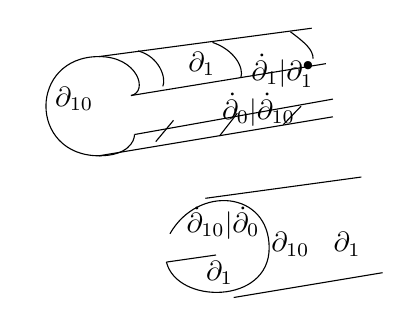
\begin{tikzpicture}[x=1cm,y=1cm,scale=.9]
\draw (0,2.4) .. controls (-1,2.4) and (-1,1) .. (0,1) .. controls (.4,1) and (.5,1.2) .. (.5,1.3);
\draw (0,2.4) .. controls (.55,2.4) and (.7,1.9) .. (.45,1.85);
\draw (0,2.4)--(3,2.8);\draw (.45,1.85)--(3.2,2.3);\draw (.5,1.3)--(3.3,1.8);\draw (0,1)--(3.3,1.55);
\draw (.55,2.48) .. controls (.85,2.4) and (.95,2.1) .. (.9,1.98);\draw (1.6,2.6) .. controls (1.9,2.5) and (2.05,2.25) .. (2,2.1);\draw (2.7,2.75) .. controls (2.9,2.6) and (3.02,2.5) .. (3.02,2.37);
\draw (.8,1.2)--(1.05,1.5);\draw (1.7,1.28)--(1.95,1.6);\draw (2.6,1.44)--(2.85,1.7);
\node at (-.35,1.8) {$\partial_{10}$};\node at (1.45,2.3) {$\partial_1$};\node at (2.6,2.2) {$\unsure{\dot\partial_1|\partial_1^\bullet}$};\node at (2.25,1.65) {$\unsure{\dot\partial_0|\dot\partial_{10}}$};
\draw (1,-.1) .. controls (1.4,.6) and (2.4,.5) .. (2.4,-.3) .. controls (2.4,-1.1) and (1.1,-1.1) .. (.95,-.5);
\draw (.95,-.5)--(1.65,-.4);\draw (1.5,.4)--(3.7,.7);\draw (1.9,-1)--(4,-.65);
\node at (1.75,.05) {$\unsure{\dot\partial_{10}|\dot\partial_0}$};\node at (1.7,-.65) {$\deleted{\unsure{\partial_1}}$};\node at (2.7,-.25) {$\partial_{10}$};\node at (3.5,-.25) {$\partial_1$};
\end{tikzpicture}}

\figure{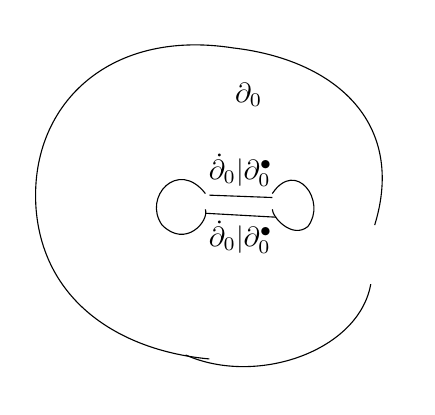
\begin{tikzpicture}[x=1cm,y=1cm]
\draw (3.8,2.1) .. controls (4.2,3.4) and (3.3,4.2) .. (2,4.35) .. controls (.4,4.6) and (-.6,3.6) .. (-.5,2.3) .. controls (-.4,1.1) and (.6,.5) .. (1.7,.4);
\draw (1.4,.45) .. controls (2.3,.05) and (3.6,.5) .. (3.75,1.35);
\draw (1.65,2.5) .. controls (1.3,2.95) and (.85,2.45) .. (1.1,2.1) .. controls (1.4,1.8) and (1.7,2.15) .. (1.65,2.3);
\draw (2.5,2.5) .. controls (2.8,2.95) and (3.2,2.4) .. (2.95,2.08) .. controls (2.75,1.92) and (2.5,2.2) .. (2.5,2.3);
\draw (1.7,2.48)--(2.5,2.45);\draw (1.65,2.25)--(2.55,2.2);
\node at (2.2,3.75) {$\partial_0$};\node at (2.1,2.8) {$\unsure{\dot\partial_0|\partial_0^\bullet}$};\node at (2.1,1.95) {$\unsure{\dot\partial_0|\partial_0^\bullet}$};
\end{tikzpicture}}

\figure{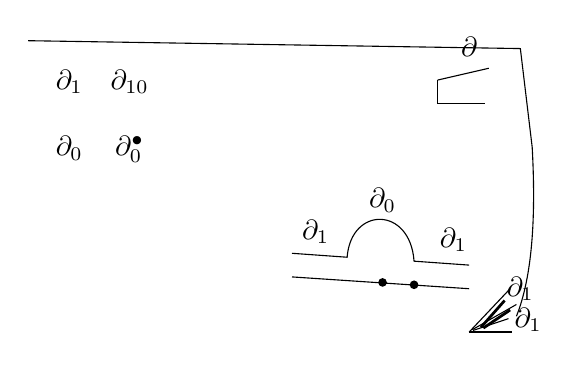
\begin{tikzpicture}[x=1cm,y=1cm]
\draw (0,3.8)--(6.25,3.7)--(6.4,2.45)..controls(6.45,1.55)and(6.4,.8)..(6.2,.3);
\node[anchor=north west] at (.05,3.6) {$\begin{array}{cc}\partial_1&\partial_{10}\\&\shortparallel\\\partial_0&\partial_0^\bullet\end{array}$};
\draw (5.2,3.3)--(5.85,3.45);\draw (5.2,3.3)--(5.2,3.0)--(5.8,3.0);\node[above] at (5.6,3.48) {$\partial$};
\draw (3.35,1.1)--(4.05,1.05)..controls(4.1,1.7)and(4.85,1.7)..(4.9,1.0)--(5.6,.95);\draw (3.35,.8)--(5.6,.65);
\fill (4.5,.73) circle(.055);\fill (4.9,.7) circle(.055);
\node[above] at (3.65,1.1) {$\partial_1$};\node[above] at (4.5,1.5) {$\partial_0$};\node[above] at (5.4,1) {$\partial_1$};
\draw (5.6,.1)--(6.15,.1);\draw (5.6,.1)--(6.12,.65);\draw (5.64,.13)--(6.2,.45);\draw (5.65,.12)--(6.1,.27);\draw[line width=1pt] (5.75,.16)--(6.05,.5);\draw[line width=1pt] (5.78,.15)--(6.12,.38);
\node at (6.25,.65) {$\partial_1$};\node at (6.35,.25) {$\deleted{\unsure{\partial_1}}$};
\end{tikzpicture}}
\mspage{42}
